\chapter{微生物代谢与生物膜}\label{ch:b2:microbial-metabolism}

取一只玻璃圆柱瓶，装入池塘淤泥、少量碎纸、一个
蛋黄和水，放在窗台上。数周之内，它
便分层形成彩色条带：顶层为绿藻，其下为铁锈色
层、一条紫色带、较低处的一条绿色带，以及
底部的黑色硫化物淤泥。除光照外未加入任何东西。每一条带都是一个种群，
各自依靠不同的化学物质生存——依靠氧气、依靠硝酸盐、依靠
硫酸盐、依靠硫化物、依靠氢气——并且每一层都为下一层提供物质。这个
柱子即是微生物世界的缩影：细胞从几乎任意一对
能够交换电子的物质中获取能量，
它们共同推动着地球的
化学循环。本章阐述这一能量学的逻辑、
微生物生长的动力学，以及微生物在表面上的群体生活，
这正是大多数微生物的实际生存方式。

\section{生存方式}

\begin{definition}[营养类型]\label{def:b2:microbial-metabolism:trophic}
\index{化能营养生物}\index{光能营养生物}\index{无机营养生物}\index{有机营养生物}
依据三个问题的答案对生物体分类。其\emph{能源}：
光（\emph{光能营养生物}）或化学反应（\emph{化能营养生物}）。
其\emph{电子来源}：无机物质——$\mathrm{H_2}$、
$\mathrm{H_2S}$、$\mathrm{NH_4^+}$、$\mathrm{Fe^{2+}}$、水——
（\emph{无机营养生物}）或有机分子（\emph{有机营养生物}）。其
\emph{碳源}：$\mathrm{CO_2}$（\emph{自养生物}）或有机
碳（\emph{异养生物}）。植物与蓝细菌是
光能无机自养生物；动物、真菌和\emph{E.~coli}是
化能有机异养生物；硝化细菌和硫氧化
细菌是化能无机自养生物，其有机物质
由$\mathrm{CO_2}$合成，能量取自
矿物的氧化，且在黑暗中进行。几乎所有组合都存在于
\omterm{def:b2:unicellular-diversity:prokaryote}{原核生物}之中；真核生物只占其中两种。
\end{definition}

\begin{theorem}[氧化还原对的能量]\label{thm:b2:microbial-metabolism:redox}
\index{氧化还原电位}\index{电子塔}
每一种产能代谢都将电子从
\emph{施主}电对转移至\emph{受主}电对。每一电对都有
标准电极电势 $E^{\circ\prime}$（pH 为 7 时），电势越负，
则越容易给出电子。将 $n$ 摩尔电子
由电势为 $E_d$ 的施主转移到电势为 $E_a$ 的受主，释放
标准自由能
\[
\Delta G^{\circ\prime} = -\,n F\,(E_a - E_d), \qquad F = \qty{96.5}{kJ/V/mol},
\]
因此产能正比于两电对之间的竖直距离，
两电对位于\emph{\omterm{thm:b2:microbial-metabolism:redox}{电子塔}}上。以
$\mathrm{O_2/H_2O}$ 的电势为 \qty{+0.82}{V}，$\mathrm{CO_2}$/葡萄糖的电势为
\qty{-0.43}{V}时，一分子葡萄糖的 24 个电子可产生
$24\times 96.5\times 1.25 = \qty{2900}{kJ/mol}$；若改将其交给
硫酸盐（$\mathrm{SO_4^{2-}/H_2S}$，\qty{-0.22}{V}），同样的
电子只能产生 $24\times 96.5\times 0.21 = \qty{490}{kJ/mol}$。
\end{theorem}
\begin{proof}
对于反应施主$_{\text{还原态}}$ + 受主$_{\text{氧化态}}$
$\to$ 施主$_{\text{氧化态}}$ + 受主$_{\text{还原态}}$，自由能
变化量即 $n$ 摩尔电子电荷 $nF$ 所做的功，
沿电势差 $E_a - E_d$ 下降，符号约定
为：自发转移（电子流向电势更正的电对）时，
有 $\Delta G < 0$。此即本科一年级分册中的能斯特关系
在两个半反应上的应用。
\end{proof}

\begin{omfigure}
\begin{tikzpicture}[every node/.style={font=\scriptsize}, y=6cm]
  \draw[thick, ->] (0,-0.55) -- (0,0.95) node[above] {$E^{\circ\prime}$ (V)};
  \foreach \v in {-0.4,-0.2,0,0.2,0.4,0.6,0.8} \draw (-0.08,\v) -- (0.08,\v) node[right, xshift=0.05cm] {\v};
  % donors on the right: value/label position/text
  \foreach \v/\y/\l in {-0.43/-0.49/{$\mathrm{CO_2}$/glucose}, -0.42/-0.40/{$2\mathrm{H^+/H_2}$}, -0.32/-0.31/{$\mathrm{NAD^+/NADH}$}, -0.27/-0.22/{$\mathrm{S^0/H_2S}$}, 0.03/0.03/{fumarate/succinate}, 0.34/0.34/{$\mathrm{NO_2^-/NH_4^+}$}}
    { \draw[omDef, thick] (0.8,\v) -- (1.6,\v); \draw[omDef] (1.6,\v) -- (1.85,\y); \node[omDef, anchor=west] at (1.9,\y) {\l}; }
  % acceptors on the left
  \foreach \v/\y/\l in {-0.24/-0.29/{$\mathrm{CO_2/CH_4}$}, -0.22/-0.17/{$\mathrm{SO_4^{2-}/H_2S}$}, 0.43/0.43/{$\mathrm{NO_3^-/NO_2^-}$}, 0.74/0.69/{$\mathrm{NO_3^-/N_2}$}, 0.77/0.77/{$\mathrm{Fe^{3+}/Fe^{2+}}$}, 0.82/0.86/{$\mathrm{O_2/H_2O}$}}
    { \draw[omThm, thick] (-1.6,\v) -- (-0.8,\v); \draw[omThm] (-1.6,\v) -- (-1.85,\y); \node[omThm, anchor=east] at (-1.9,\y) {\l}; }
  \node[omThm, anchor=south] at (-2.4,0.93) {受主};
  \node[omDef, anchor=south] at (2.4,0.93) {施主};
  % arrows showing two metabolisms
  \draw[->, very thick, omExo!80!black] (4.9,-0.43) -- (4.9,0.80);
  \node[anchor=west, align=left] at (5.0,0.2) {有氧呼吸 \\葡萄糖：\qty{1.25}{V}，\\\qty{2900}{kJ/mol}};
  \draw[->, very thick, omProp] (4.2,-0.43) -- (4.2,-0.24);
  \node[anchor=north, align=center] at (4.2,-0.52) {硫酸盐还原：\\\qty{0.21}{V}，\qty{490}{kJ/mol}};
  \draw[dashed, gray] (3.5,-0.43) -- (4.9,-0.43);
  \draw[dashed, gray] (3.5,0.82) -- (4.9,0.82);
  \draw[dashed, gray] (3.5,-0.22) -- (4.2,-0.22);
\end{tikzpicture}

{\small \omterm{thm:b2:microbial-metabolism:redox}{电子塔}。施主（蓝色）按其
标准电势列出；受主（红色）同样如此。代谢过程即是由施主
落至位于其上方的受主，其能量产出
与下落高度成正比：葡萄糖到氧气是一段
长距离的下落，葡萄糖到硫酸盐则是一段短距离的下落。}
\end{omfigure}

\begin{proposition}[化能无机营养]\label{prop:b2:microbial-metabolism:lithotrophy}
\index{化能无机营养}\index{硝化作用}
一些细菌的全部能量来自无机物的氧化，并以
氧气（或硝酸盐）为受主，并固定 $\mathrm{CO_2}$，所用
的 ATP 与还原力皆由此获得。\emph{硝化细菌}：铵
氧化菌（\emph{Nitrosomonas}）将 $\mathrm{NH_4^+}$ 转化为亚硝酸盐
（$\Delta G^{\circ\prime} = \qty{-275}{kJ/mol}$），亚硝酸盐氧化菌
（\emph{Nitrobacter}）将亚硝酸盐转化为硝酸盐（\qty{-74}{kJ/mol}）；
二者共同将分解产生的铵转化为
植物吸收的硝酸盐（\cref{ch:b2:biogeochemical-cycles}）。
\emph{硫氧化菌}（\emph{Thiobacillus}、\emph{Beggiatoa}）
将 $\mathrm{H_2S}$ 氧化为硫和硫酸盐；\emph{铁氧化菌}
将 $\mathrm{Fe^{2+}}$ 氧化为铁锈；\emph{氢氧化菌}燃烧
$\mathrm{H_2}$。由于它们的电子施主位于\omterm{thm:b2:microbial-metabolism:redox}{电子塔}的高处，
每分子的产能很少，又因为它们的施主是比
NADH 更弱的还原剂，它们必须耗费能量，驱使电子
\emph{逆行}，以生成碳固定所需的 NADH：
一个硝化细菌须氧化约三十个铵离子，才能固定一
$\mathrm{CO_2}$，且生长缓慢。
\end{proposition}
\begin{proof}[证据]
维诺格拉茨基（1887--1890）在一滴水中培养丝状硫细菌，他让
硫化物从一侧扩散进来，空气则从另一侧扩散进来：细菌
聚集在边界处，积累硫
粒，并在硫化物被切断后将其消耗掉。
随后，他在纯无机培养基上分离出硝化细菌，该培养基含有
铵，完全不含有机碳，细菌在其上生长并
产生硝酸盐——这首次证明生命可以
由 $\mathrm{CO_2}$ 与无机反应释放的能量构建，
无需光照。他称之为化能合成。
\end{proof}

\begin{omfigure}
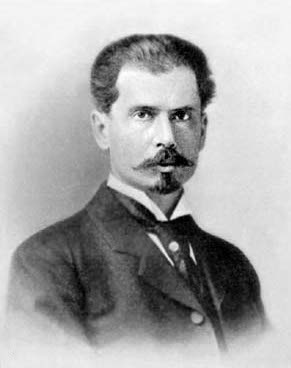
\includegraphics[width=0.26\linewidth]{images/book4/winogradsky.jpg}\hspace{0.05\linewidth}
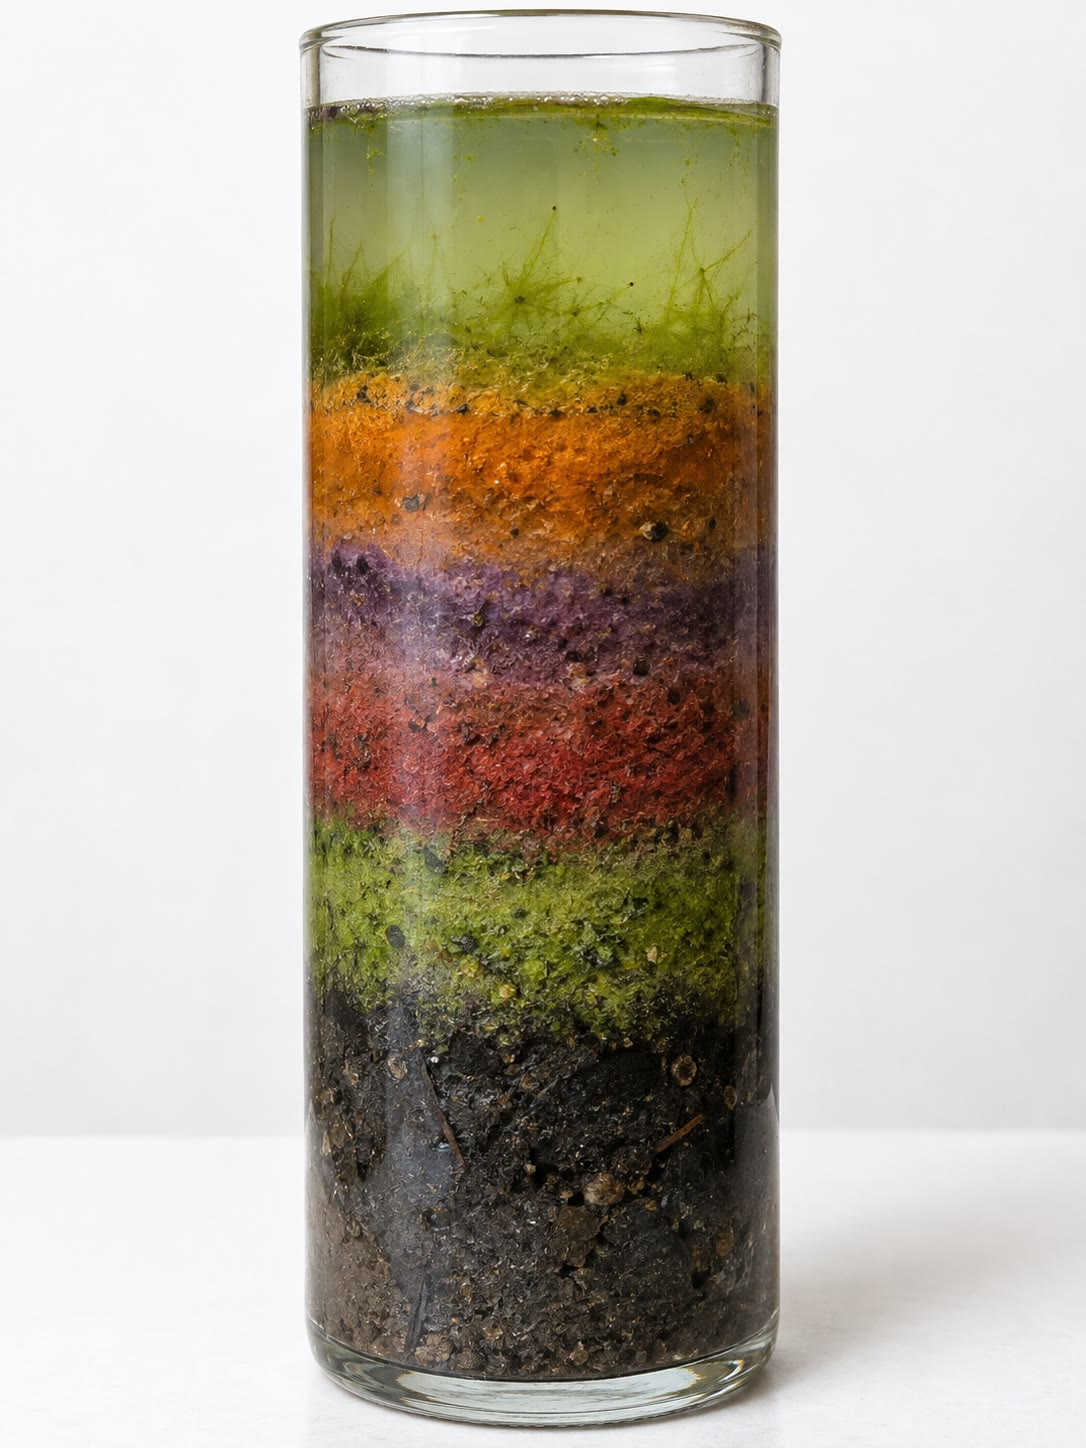
\includegraphics[width=0.30\linewidth]{images/book4/ai/b4-02-winogradsky-column.jpg}

{\small 谢尔盖·维诺格拉茨基，\omterm{prop:b2:microbial-metabolism:lithotrophy}{化能无机营养}的发现者，以及以他命名的
柱：一个由泥与水组成的圆柱，在光照下分层形成
藻类、铁与硫的氧化菌、紫色和绿色硫细菌的条带，
以及黑色泥中的\omterm{def:b2:microbial-metabolism:anaerobic}{硫酸盐还原}菌。}
\end{omfigure}

\begin{definition}[不产氧光合作用]\label{def:b2:microbial-metabolism:anoxygenic}
\index{不产氧光合作用}
紫色和绿色细菌进行光合作用时只用一个
光系统及一种吸收近红外光的细菌叶绿素，
以 $\mathrm{H_2S}$、$\mathrm{H_2}$ 或有机酸代替水作为电子供体：
它们释放硫或硫酸盐，从不释放氧气，
并且所需光的波长须能穿过其上方的
绿色与蓝细菌层。因此紫色硫细菌
生长在维诺格拉茨基柱的紫色带中，
正处于来自下方的硫化物与来自上方的光相遇之处；
绿色硫细菌耐受更多硫化物、所需光照更少，生长在它们下方，
产氧光合作用具有两个串联的光系统，
是后来某一谱系——蓝细菌——的发明，
——它学会了从水中夺取电子。
\end{definition}

\section{厌氧呼吸与发酵}

\begin{definition}[厌氧呼吸]\label{def:b2:microbial-metabolism:anaerobic}
\index{厌氧呼吸}\index{反硝化作用}\index{硫酸盐还原}\index{产甲烷作用}
\emph{厌氧呼吸}是一种呼吸作用——一条电子传递链，
通过化学渗透泵出质子并合成 ATP，其末端
受体不是氧。\emph{反硝化细菌}
（\emph{Pseudomonas}、\emph{Paracoccus}）将硝酸盐还原为亚硝酸盐、
一氧化氮、一氧化二氮，最终还原为 $\mathrm{N_2}$，它逸入
空气中；它们利用其有氧呼吸链并加入少量额外的酶，
只有在氧气耗尽时才转而利用硝酸盐。\emph{硫酸盐
还原菌}（\emph{Desulfovibrio}）将硫酸盐还原为硫化物，使
泥变黑，并使其带有臭味。\emph{产甲烷菌}，
属于古菌，以 $\mathrm{CO_2}$ 与 $\mathrm{H_2}$ 反应生成
甲烷（$4\mathrm{H_2} + \mathrm{CO_2} \to \mathrm{CH_4} +
2\mathrm{H_2O}$，$\Delta G^{\circ\prime} = \qty{-131}{kJ/mol}$），或
将乙酸分解为甲烷和 $\mathrm{CO_2}$；它们会被
氧气杀死，生活在牛瘤胃、稻田、沼泽和垃圾填埋场中，
它们释放的一种温室气体，正是
\cref{ch:b2:global-change}所讨论的内容。铁和锰的氧化物则为其他
类群所利用。本科一年级分册将氧气视为\emph{唯一}的受体；就
地球历史的大部分时期，以及今天的每一层沉积物而言，它只是
一系列受体中的第一个。
\end{definition}

\begin{proposition}[沉积物中电子受体的顺序]\label{prop:b2:microbial-metabolism:sequence}
向下穿过饱水沉积物时，电子受体
按其所释放能量的顺序被耗尽：氧气位于
最上层的数毫米，其次是硝酸盐，再次是锰和铁的氧化物，
然后是硫酸盐，最后是 $\mathrm{CO_2}$（\omterm{def:b2:microbial-metabolism:anaerobic}{产甲烷作用}）所在的
最深的缺氧层。这一顺序即“能量塔”的次序：在每一深度，
利用剩余最优受体的生物生长最快，
与其他类群争夺有机供体，并在
耗尽其受体后，下一类群接手。在海洋中，硫酸盐
丰富（\qty{28}{mmol/L}），硫酸盐带很厚，\omterm{def:b2:microbial-metabolism:anaerobic}{产甲烷作用}
仅在深数米处才开始；而在淡水沼泽中，
因硫酸盐贫乏，甲烷在表层之下即形成。
\end{proposition}

\begin{omfigure}
\begin{tikzpicture}[every node/.style={font=\scriptsize}]
  \fill[omDef!8] (0,0) rectangle (4,0.6);
  \node at (2,0.3) {水};
  \fill[omExo!35] (0,-0.5) rectangle (4,0);
  \fill[omProp!25] (0,-1.3) rectangle (4,-0.5);
  \fill[omProp!45] (0,-2.0) rectangle (4,-1.3);
  \fill[gray!50] (0,-3.4) rectangle (4,-2.0);
  \fill[black!75] (0,-4.4) rectangle (4,-3.4);
  \draw[thick] (0,0.6) -- (0,-4.4); \draw[thick] (4,0.6) -- (4,-4.4);
  \draw[thick] (0,0) -- (4,0);
  \node[anchor=west, align=left] at (4.2,-0.25) {有氧呼吸：$\mathrm{O_2 \to H_2O}$——\qty{2.9}{MJ} 每葡萄糖};
  \node[anchor=west, align=left] at (4.2,-0.9) {硝酸盐还原：$\mathrm{NO_3^- \to N_2}$——\qty{2.7}{MJ}};
  \node[anchor=west, align=left] at (4.2,-1.65) {锰和铁还原：$\mathrm{Fe^{3+} \to Fe^{2+}}$};
  \node[anchor=west, align=left, white] at (0.1,-2.7) {};
  \node[anchor=west, align=left] at (4.2,-2.7) {硫酸盐还原：$\mathrm{SO_4^{2-} \to H_2S}$——\qty{0.5}{MJ}};
  \node[anchor=west, align=left] at (4.2,-3.9) {产甲烷作用：$\mathrm{CO_2 \to CH_4}$——\qty{0.4}{MJ}};
  \draw[->, thick] (-0.5,0) -- (-0.5,-4.4) node[below] {深度};
  \node[anchor=east] at (-0.6,-0.25) {mm};
  \node[anchor=east] at (-0.6,-2.7) {cm 至 m};
\end{tikzpicture}

{\small 沉积物中电子受体随深度的
演替，按每葡萄糖所释放的能量排列。每
一带中的生物与下一带竞争有机物，直至其
受体耗尽。}
\end{omfigure}

\begin{definition}[发酵（再论）]\label{def:b2:microbial-metabolism:fermentation}
\index{发酵!微生物}
\emph{发酵}不使用外部受体：有机
底物分解为一种氧化程度较高的产物和一种还原程度较高的产物，
ATP 仅通过底物水平磷酸化产生，而糖酵解的 NADH
通过还原一种代谢物而被重新氧化。酵母产生
乙醇和 $\mathrm{CO_2}$；乳酸菌产生乳酸（酸奶、
酸菜、肌肉酸痛）；\emph{E.~coli} 产生混合酸、
乙醇和气体；梭菌产生丁酸盐、丁醇和丙酮；
丙酸杆菌产生瑞士奶酪中的丙酸盐和
$\mathrm{CO_2}$。发酵每葡萄糖得两个 ATP，呼吸作用则约得三十个，
故发酵者须多处理十五倍的糖，
方能获得相同的生长量，且其产物——酸与酒精——毒害
自身所处的培养基：发酵之所以能保存食物，是因为发酵者
使食物不再适于生存，连它自身也不例外。
\end{definition}

\begin{example}[互养：靠剩余物生活]\label{ex:b2:microbial-metabolism:syntrophy}
在缺氧沉积物中，\omterm{def:b2:microbial-metabolism:fermentation}{发酵}菌留下乙酸盐、丙酸盐、
丁酸盐和 $\mathrm{H_2}$。将丙酸盐氧化为乙酸盐和
$\mathrm{H_2}$ 的反应，其标准自由能为\emph{正}值，
（\qty{+76}{kJ/mol}），本不可能发生——除非旁边的产甲烷菌
随生随耗地消耗氢气，使其分压保持在
\qty{1e-4}{atm} 以下，此时反应方能成为
放能的。两者单独都无法以丙酸盐为底物生长；二者合作，
便将其转化为甲烷。这种\emph{种间氢
转移}正是厌氧消化总由菌群协作完成的原因，
也是古菌与其细菌伙伴常常
紧贴在一起被发现的原因。
\end{example}

\section{底物上的生长}

\begin{theorem}[莫诺定律]\label{thm:b2:microbial-metabolism:monod}
\index{莫诺方程}\index{产量系数}
在单一限制性底物上生长的种群，
浓度为 $S$ 时，其比生长速率为
\[
\mu = \mu_{\max}\,\frac{S}{K_s + S}, \qquad \frac{\mathrm{d}X}{\mathrm{d}t} = \mu X,
\]
其中 $X$ 为生物量浓度，$\mu_{\max}$ 为最大
速率（等于最短\omterm{def:b2:unicellular-diversity:division}{世代时间}的倒数除以
$\ln 2$），$K_s$ 为\emph{半饱和常数}，
即生长速率达到一半时的底物浓度——对\emph{E.~coli}而言，
葡萄糖浓度仅为每升几毫克。底物的消耗与生长成正比，
$\mathrm{d}S/\mathrm{d}t =
-\mu X/Y$，其中 $Y$ 为\emph{产量}：每克底物所产生的生物量克数，
有氧条件下以糖为底物时约为 \num{0.5}，
\omterm{def:b2:microbial-metabolism:fermentation}{发酵}者则约为 \num{0.1}。
\end{theorem}
\begin{proof}[证据]
莫诺（1942 年）在一系列葡萄糖浓度下分批培养\emph{E.~coli}，
并测定各浓度下的指数生长速率：
速率随浓度升高而上升并趋于饱和，呈米氏曲线形状，
这正是速率由可饱和的摄取系统决定时所预期的结果。
该定律是经验性的——细胞内有成千上万种酶，而非一种——
但它几乎符合所有受底物限制的培养，
也是\omterm{def:b2:microbial-metabolism:fermentation}{发酵}工艺和
废水工程的基础。
\end{proof}

\begin{theorem}[恒化器]\label{thm:b2:microbial-metabolism:chemostat}
\index{恒化器}\index{稀释速率}
\emph{\omterm{thm:b2:microbial-metabolism:chemostat}{恒化器}}是一个体积为 $V$ 的容器，持续加入新鲜培养基
（底物浓度为 $S_{\text{入}}$），以流量 $F$ 注入并以相同流量排出，
因此\emph{\omterm{thm:b2:microbial-metabolism:chemostat}{稀释速率}}为 $D = F/V$。生物量与
底物满足
\[
\frac{\mathrm{d}X}{\mathrm{d}t} = (\mu - D)\,X, \qquad
\frac{\mathrm{d}S}{\mathrm{d}t} = D\,(S_{\text{入}} - S) - \frac{\mu X}{Y}.
\]
在稳态下 $\mu = D$：培养物的生长速率恰好等于其被冲出的速率，
只要 $D$ 低于某一临界值，无论取何值均如此，
操作者通过调节泵即可设定生长速率。稳态时的
底物浓度与生物量为
\[
S^* = \frac{K_s\,D}{\mu_{\max} - D}, \qquad X^* = Y\,(S_{\text{入}} - S^*),
\]
而当\omterm{thm:b2:microbial-metabolism:chemostat}{稀释速率}超过\emph{冲出}速率 $D_c = \mu_{\max}
S_{\text{入}}/(K_s + S_{\text{入}})$ 时，任何种群都无法维持。
\end{theorem}
\begin{proof}
令 $\mathrm{d}X/\mathrm{d}t = 0$ 且 $X \neq 0$，得 $\mu = D$；
将莫诺定律反解，得 $D(K_s + S^*) = \mu_{\max} S^*$，从而 $S^* =
K_s D/(\mu_{\max} - D)$。令 $\mathrm{d}S/\mathrm{d}t = 0$，
并将 $\mu$ 换成 $D$：$D(S_{\text{入}} - S^*) = DX^*/Y$，由此
得 $X^*$。解仅在 $S^* < S_{\text{入}}$ 时存在，即\
$D < \mu_{\max} S_{\text{入}}/(K_s + S_{\text{入}})$；超过此值后，
则 $\mu < D$ 对任意 $S \le S_{\text{入}}$ 成立，$X$ 衰减至零。
该稳态是稳定的：若 $X$ 上升，则 $S$ 下降，$\mu$ 降至
$D$ 以下，$X$ 又被冲回。
\end{proof}

\begin{omfigure}
\begin{minipage}[b]{0.48\linewidth}\centering
\begin{tikzpicture}
\begin{axis}[
  width=0.94\linewidth, height=5.4cm,
  axis x line=bottom, axis y line=left,
  xmin=0, xmax=0.5, ymin=0, ymax=1.1,
  xlabel={$S$ (\unit{g/L})}, ylabel={$\mu$ (\unit{h^{-1}})},
  xlabel style={font=\small, at={(axis description cs:0.5,-0.14)}, anchor=north},
  ylabel style={font=\small},
  tick label style={font=\small}, xtick={0,0.1,0.2,0.3,0.4,0.5}, ytick={0,0.5,1},
  clip=false,
]
\addplot[very thick, omDef, domain=0:0.5, samples=100] {x/(0.02+x)};
\draw[dashed, gray] (axis cs:0,1) -- (axis cs:0.5,1); \node[font=\scriptsize, anchor=south east] at (axis cs:0.5,1) {$\mu_{\max}$};
\draw[dashed, gray] (axis cs:0,0.5) -- (axis cs:0.02,0.5) -- (axis cs:0.02,0); \node[font=\scriptsize, anchor=north west] at (axis cs:0.02,-0.02) {$K_s$};
\end{axis}
\end{tikzpicture}
\end{minipage}\hfill
\begin{minipage}[b]{0.5\linewidth}\centering
\begin{tikzpicture}
\begin{axis}[
  width=0.94\linewidth, height=5.4cm,
  axis x line=bottom, axis y line=left,
  xmin=0, xmax=1.1, ymin=0, ymax=2.2,
  xlabel={稀释速率 $D$ (\unit{h^{-1}})}, ylabel={\unit{g/L}},
  xlabel style={font=\small, at={(axis description cs:0.5,-0.14)}, anchor=north},
  ylabel style={font=\small},
  tick label style={font=\small}, xtick={0,0.5,1}, ytick={0,1,2},
  legend style={font=\scriptsize, at={(0.05,0.62)}, anchor=west, draw=none},
  clip=false,
]
\addplot[very thick, omDef, domain=0:0.99, samples=200] {0.5*(2 - 0.02*x/(1-x))};
\addlegendentry{生物量 $X^*$}
\addplot[very thick, omThm, domain=0:0.99, samples=200] {0.02*x/(1-x)};
\addlegendentry{底物 $S^*$}
\addplot[thick, omProp, dashed, domain=0:0.99, samples=200] {x*0.5*(2 - 0.02*x/(1-x))};
\addlegendentry{输出 $D X^*$}
\draw[dashed, gray] (axis cs:0.99,0) -- (axis cs:0.99,2.1); \node[font=\scriptsize, anchor=south, align=center] at (axis cs:0.9,2.1) {冲出};
\end{axis}
\end{tikzpicture}
\end{minipage}

{\small 左图：莫诺定律，$\mu_{\max} = \qty{1}{h^{-1}}$，
$K_s = \qty{0.02}{g/L}$。右图：\omterm{thm:b2:microbial-metabolism:chemostat}{恒化器}以
\qty{2}{g/L} 的底物进料（$Y = 0.5$）：生物量几乎
保持恒定，残余底物直至冲出速率前都几乎为零，
在冲出速率附近底物穿透，
种群随之崩溃；每小时的生物量输出在此之前最大。}
\end{omfigure}

\begin{omfigure}
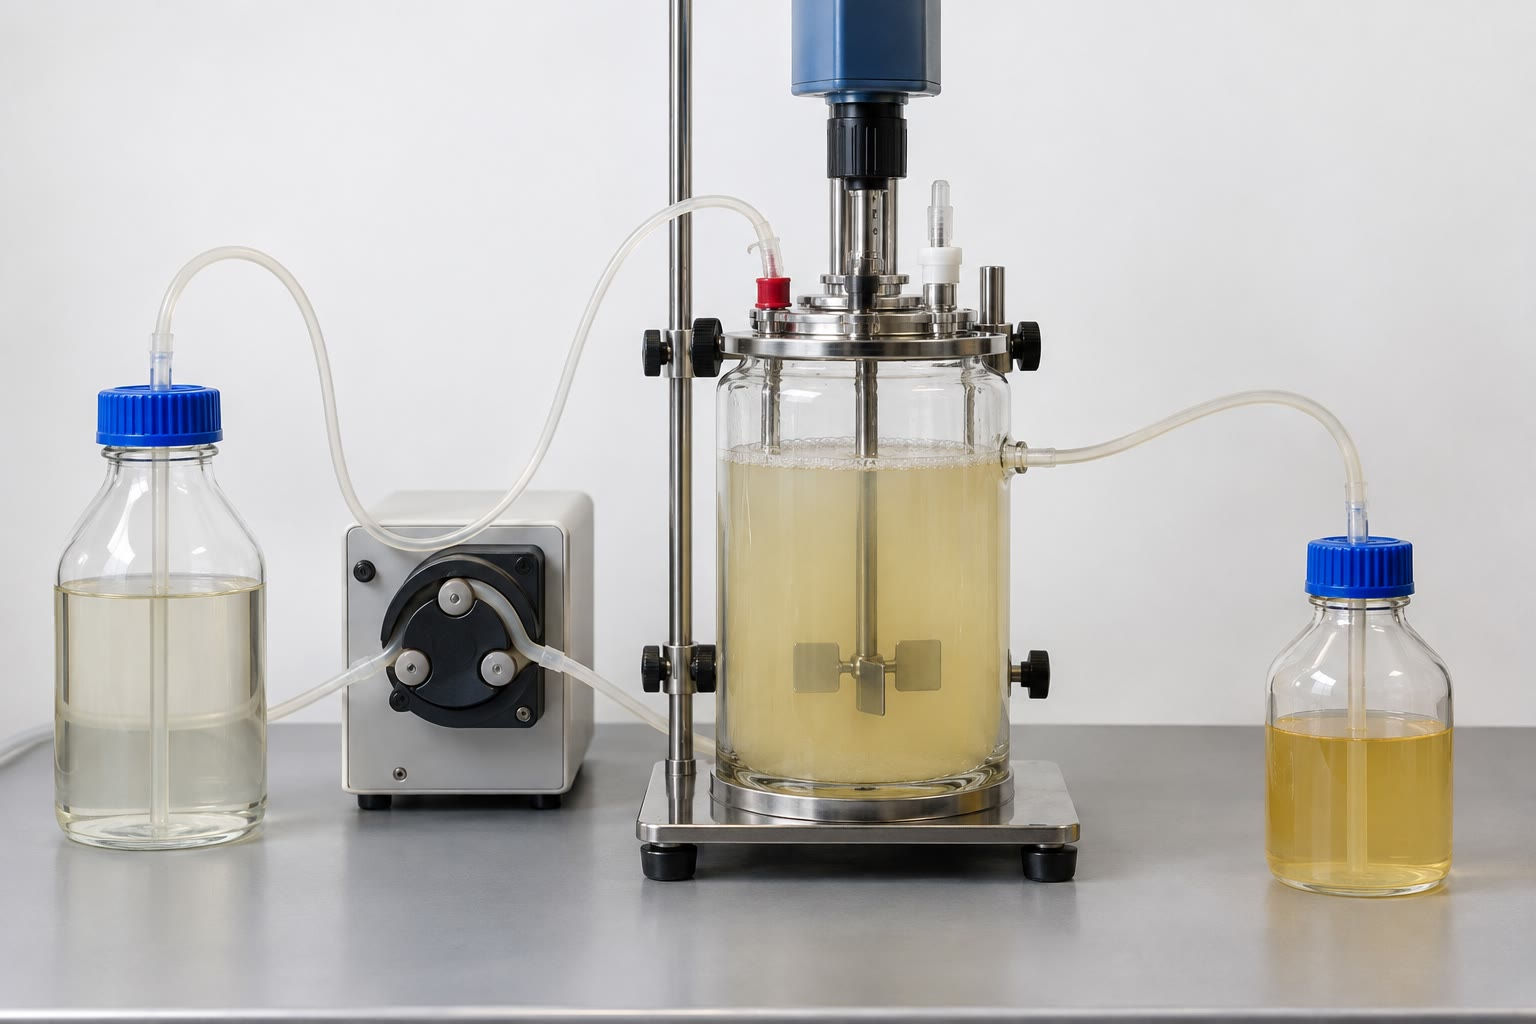
\includegraphics[width=0.6\linewidth]{images/book4/ai/b4-02-chemostat.jpg}

{\small 实验室\omterm{thm:b2:microbial-metabolism:chemostat}{恒化器}：新鲜培养基由
左侧的储库泵入，培养物从右侧溢出；
泵的流速决定生长速率。}
\end{omfigure}

\begin{example}[读取恒化器]\label{ex:b2:microbial-metabolism:chemostat}
取 $\mu_{\max} = \qty{1.0}{h^{-1}}$，$K_s = \qty{0.02}{g/L}$，
$S_{\text{入}} = \qty{2}{g/L}$，$Y = 0.5$，当 $D =
\qty{0.5}{h^{-1}}$ 时：$S^* = 0.02\times 0.5/0.5 = \qty{0.02}{g/L}$，
$X^* = 0.5\times 1.98 = \qty{0.99}{g/L}$；培养物留下未被利用的糖，
占 \qty{1}{\%}。冲出速率为 $1.0\times
2/2.02 = \qty{0.99}{h^{-1}}$。消化器或肠道遵循同一原理：
人的结肠每天进食三次、排空一次，
细菌在接近 \qty{0.04}{h^{-1}} 的\omterm{thm:b2:microbial-metabolism:chemostat}{稀释速率}下得以保持，任何
不能在一天内倍增的物种都会被冲走——除非
它附着在肠壁上。
\end{example}

\section{生物膜}

\begin{definition}[生物膜]\label{def:b2:microbial-metabolism:biofilm}
\index{生物膜}\index{细胞外基质!细菌的}
\emph{生物膜}是附着于表面的微生物群落，
包埋于自身分泌的\emph{基质}之中，基质由多糖、
蛋白质和胞外 DNA 组成。它分阶段形成：
单个细胞可逆地\emph{附着}（借助鞭毛、菌毛），
不可逆附着并生长形成\emph{微菌落}，\emph{成熟}为
具有菌柱和水道的结构化膜，并
最后细胞\emph{扩散}，游离而去，在新的表面定居。
基质保存水分和营养物质，保护细胞免于
干燥、捕食者、抗生素和免疫细胞的侵害，并建立
化学梯度，使膜成为由多种生态位构成的景观。地球上的大多数
细菌以这种方式生活：在溪流中的岩石上、根上、
牙齿上（牙菌斑）、导管和植入物上、囊性纤维化患者的肺中、
船体上以及管道中。
\end{definition}

\begin{omfigure}
\begin{tikzpicture}[every node/.style={font=\scriptsize}]
  \fill[gray!35] (0,0) rectangle (13.6,0.35);
  \node at (6.8,0.17) {表面};
  % stage 1 attachment
  \foreach \p in {(0.6,0.55),(1.4,0.55)} \draw[thick, omDef, fill=omDef!30] \p ellipse (0.22 and 0.1);
  \draw[thick, omDef, fill=omDef!30] (1.0,1.6) ellipse (0.22 and 0.1);
  \draw[->, omDef] (1.0,1.45) -- (1.0,0.75);
  \node[below, align=center] at (1.1,-0.05) {1. 附着};
  % stage 2 microcolony
  \begin{scope}[xshift=3.4cm]
    \fill[omExo!25] (0.15,0.35) .. controls (0.1,1.1) and (1.5,1.1) .. (1.45,0.35);
    \foreach \p in {(0.45,0.5),(0.8,0.5),(1.15,0.5),(0.6,0.75),(0.95,0.75),(0.8,0.95)} \draw[thick, omDef, fill=omDef!30] \p ellipse (0.18 and 0.09);
    \node[below, align=center] at (0.8,-0.05) {2. 微菌落，\\分泌基质};
  \end{scope}
  % stage 3 mature with channels
  \begin{scope}[xshift=6.8cm]
    \fill[omExo!25] (0.0,0.35) .. controls (0.2,1.9) and (0.9,2.2) .. (1.1,1.5) .. controls (1.2,0.9) and (1.4,0.6) .. (1.5,0.35);
    \fill[omExo!25] (1.7,0.35) .. controls (1.6,1.5) and (2.6,2.3) .. (2.9,1.2) .. controls (3.0,0.8) and (3.1,0.5) .. (3.2,0.35);
    \foreach \p in {(0.35,0.55),(0.7,0.55),(0.5,0.85),(0.8,1.15),(0.55,1.45),(2.0,0.6),(2.4,0.6),(2.2,0.9),(2.5,1.25),(2.3,1.6),(2.6,1.9),(2.1,1.3)} \draw[thick, omDef, fill=omDef!30] \p ellipse (0.16 and 0.08);
    \draw[<->, omThm, thick] (1.6,0.5) -- (1.6,1.6);
    \node[omThm, anchor=south] at (1.6,2.45) {水道};
    \node[below, align=center] at (1.6,-0.05) {3. 成熟膜：菌柱，\\水道，梯度};
  \end{scope}
  % stage 4 dispersal
  \begin{scope}[xshift=11.2cm]
    \fill[omExo!25] (0.0,0.35) .. controls (0.1,1.5) and (1.0,1.6) .. (1.1,0.35);
    \foreach \p in {(0.3,0.55),(0.65,0.55),(0.5,0.85)} \draw[thick, omDef, fill=omDef!30] \p ellipse (0.16 and 0.08);
    \foreach \p/\a in {(1.4,1.5)/40,(1.9,1.1)/10,(1.6,2.0)/70} \draw[thick, omDef, fill=omDef!30, rotate around={\a:\p}] \p ellipse (0.16 and 0.08);
    \draw[->, omDef] (1.0,1.0) -- (1.35,1.35);
    \node[below, align=center] at (1.0,-0.05) {4. 扩散};
  \end{scope}
\end{tikzpicture}

{\small \omterm{def:b2:microbial-metabolism:biofilm}{生物膜}的生命周期：单个细胞附着，生长为
分泌基质（灰色）的微菌落，成熟为
具有菌柱和水道的结构化膜，并释放
游动细胞，在新的表面定殖。}
\end{omfigure}

\begin{omfigure}
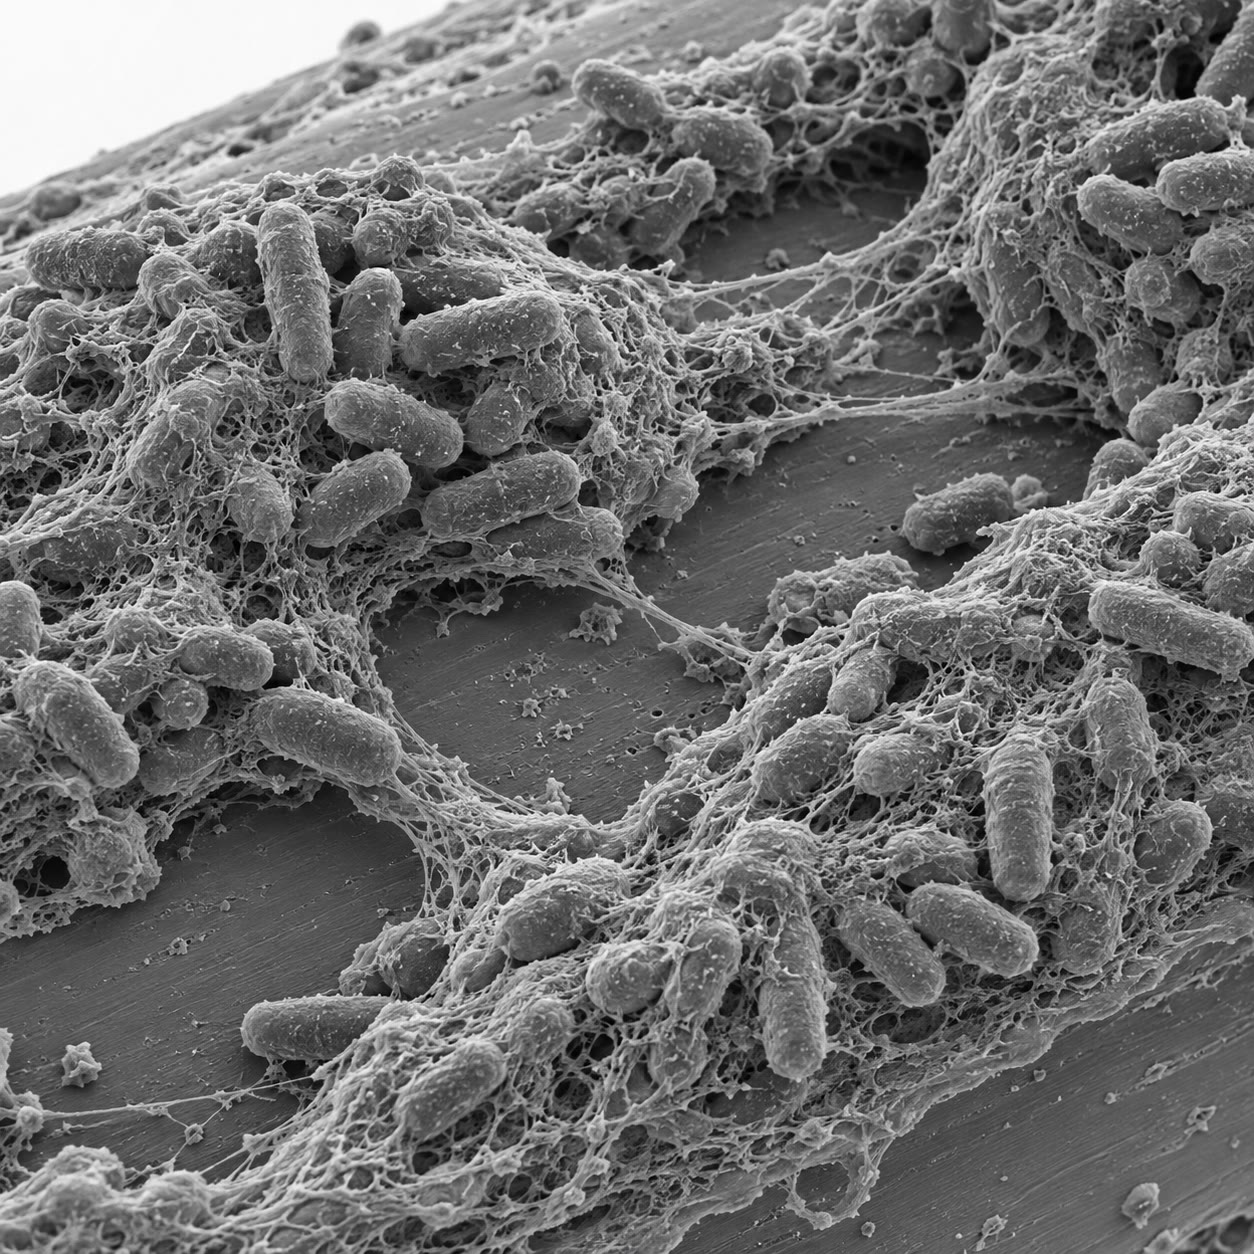
\includegraphics[width=0.46\linewidth]{images/book4/ai/b4-02-biofilm-sem.jpg}

{\small 导管上的\omterm{def:b2:microbial-metabolism:biofilm}{生物膜}，经扫描电子显微镜观察：
杆状细菌包埋于其分泌的纤维状基质中，
团簇之间有开放的水道。}
\end{omfigure}

\begin{theorem}[生物膜内的梯度]\label{thm:b2:microbial-metabolism:gradient}
\index{氧气穿透深度}
设膜的厚度为 $L$，其中细胞以恒定的体积速率 $q$ 消耗氧气，
使表面处的浓度保持为 $c_0$，
基底处无通量，则稳态氧浓度分布为
抛物线分布；若膜足够厚，以致氧气会耗尽，
则耗尽发生在\emph{穿透深度}
\[
L_p = \sqrt{\frac{2 D_e\, c_0}{q}},
\]
处，其中 $D_e$ 为基质中的有效扩散系数。
取 $D_e = \qty{1.5e-9}{m^2/s}$，$c_0 = \qty{0.25}{mol/m^3}$，且 $q
= \qty{0.17}{mol/m^3/s}$（致密的呼吸细胞膜），$L_p
\approx \qty{66}{\micro m}$：厚度低于十分之一毫米时，\omterm{def:b2:microbial-metabolism:biofilm}{生物膜}
即处于缺氧状态，反硝化细菌、\omterm{def:b2:microbial-metabolism:fermentation}{发酵}细菌和\omterm{def:b2:microbial-metabolism:anaerobic}{硫酸盐还原}菌
生活在好氧菌构成的“屋顶”之下。
\end{theorem}
\begin{proof}
设 $x$ 为表面以下的深度。在稳态下，
扩散通量 $-D_e\,\mathrm{d}c/\mathrm{d}x$ 随深度的变化
仅由消耗引起：$D_e\,\mathrm{d}^2c/\mathrm{d}x^2 = q$。
两次积分得 $c = c_0 + a x + q x^2/2D_e$。若氧气
在深度 $L_p$ 处耗尽，且该处通量为零（下方无来源），
则 $c(L_p) = 0$ 且 $c'(L_p) = 0$：由第二式得 $a = -qL_p/D_e$，
代入第一式得 $c_0 - qL_p^2/D_e + qL_p^2/2D_e = 0$，即
$L_p^2 = 2D_e c_0/q$。分布为 $c = (q/2D_e)(L_p - x)^2$。
\end{proof}

\begin{omfigure}
\begin{tikzpicture}
\begin{axis}[
  width=0.78\linewidth, height=5.6cm,
  axis x line=bottom, axis y line=left,
  xmin=0, xmax=120, ymin=0, ymax=0.28,
  xlabel={膜内深度 (\unit{\micro m})}, ylabel={$\mathrm{O_2}$ (\unit{mol/m^3})},
  xlabel style={font=\small, at={(axis description cs:0.5,-0.14)}, anchor=north},
  ylabel style={font=\small},
  tick label style={font=\small}, xtick={0,20,40,60,80,100,120}, ytick={0,0.1,0.2},
  clip=false,
]
\addplot[very thick, omDef, domain=0:66, samples=60] {0.25*(1-x/66)^2};
\addplot[very thick, omDef, domain=66:120, samples=2] {0};
\fill[omThm!12] (axis cs:66,0) rectangle (axis cs:120,0.28);
\node[font=\scriptsize, anchor=north, align=center] at (axis cs:93,0.27) {缺氧区：\\反硝化细菌、发酵菌、\\硫酸盐还原菌};
\draw[dashed, gray] (axis cs:66,0) -- (axis cs:66,0.28); \node[font=\scriptsize, anchor=south] at (axis cs:66,0.28) {$L_p$};
\node[font=\scriptsize, anchor=west] at (axis cs:24,0.18) {好氧区};
\end{axis}
\end{tikzpicture}

{\small 进行呼吸的\omterm{def:b2:microbial-metabolism:biofilm}{生物膜}内的氧气：自表面的主体值起呈抛物线下降，
至穿透深度处降为零，
\qty{66}{\micro m}为定理中的数值。更深处
均为缺氧。}
\end{omfigure}

\begin{proposition}[群体感应]\label{prop:b2:microbial-metabolism:quorum}
\index{群体感应}\index{自诱导物}
细菌能够“数”出自身的数量。每个细胞
以恒定的低速率分泌一种小分子信号，即\emph{\omterm{prop:b2:microbial-metabolism:quorum}{自诱导物}}
（革兰氏阴性菌中为酰基高丝氨酸内酯，革兰氏阳性菌中为
短肽）。在稀悬液中，信号会扩散散失；在密集的种群或\omterm{def:b2:microbial-metabolism:biofilm}{生物膜}中，
信号不断积累，当浓度超过阈值时，
它便与受体结合，从而开启一组基因
——其中包括\omterm{prop:b2:microbial-metabolism:quorum}{自诱导物}自身的基因，这也是其名称的由来。
受这一机制调控的基因，都是只有在众多细胞协同行动时才有益处的：
发光、分泌消化酶和毒素、产生基质，以及
病原体的毒力——病原体必须同时压倒宿主，
而非逐个细胞地发出警报。
\end{proposition}
\begin{proof}[证据]
Nealson、Platt 和 Hastings（1970）发现，海洋细菌
\emph{Vibrio fischeri} 能使乌贼的器官发光，在稀培养物中它不发光，
只有密度超过约 $10^{7}$ 个细胞每毫升时才会发光；
取自密集、发光培养物的无细胞培养基，能使稀培养物立即发光。
该培养基含有信号分子，其结构为酰基高丝氨酸内酯，于 1981 年被确定，
而无法合成该分子的突变体，无论密度多高，
都从不发光。
\end{proof}

\begin{example}[生物膜为何能耐受抗生素]\label{ex:b2:microbial-metabolism:tolerance}
\omterm{def:b2:microbial-metabolism:biofilm}{生物膜}中的细胞所能承受的抗生素浓度，
是能在悬浮状态下杀死同一菌株的浓度的
一百至一千倍，且无需任何抗性基因。
基质减缓药物的扩散，并结合其中一部分；
浓度梯度使深层细胞处于饥饿、缺氧且几乎不生长的状态。
而大多数抗生素只杀死正在生长的细胞（青霉素需要\omterm{def:b2:unicellular-diversity:prokaryote}{细胞壁}合成，
氨基糖苷类需要主动转运）；少数\emph{持留菌}细胞则完全处于休眠状态，
治疗停止后便会重新形成\omterm{def:b2:microbial-metabolism:biofilm}{生物膜}。因此，植入物上的慢性感染通常
需要通过取出植入物来治疗。
\end{example}

\section{微生物群落}

\begin{example}[维诺格拉茨基柱的解释]\label{ex:b2:microbial-metabolism:column}
光和空气从上方进入，
有机物和硫酸盐则来自底泥。蓝细菌和藻类
在顶部生长并释放氧气。下方的异养生物消耗有机物上的氧气，
随后消耗硝酸盐；更深处，\omterm{def:b2:microbial-metabolism:anaerobic}{硫酸盐还原}菌将硫酸盐转化为硫化物，
硫化物向上扩散，使底泥因硫化铁而变黑。在上升的硫化物
与下降的光相遇之处，紫硫细菌通过光合作用将其氧化（即紫色条带），
其下方为绿硫细菌；在硫化物与氧气相遇的黑暗处，
无色硫氧化菌（如\emph{Beggiatoa}）
以\omterm{prop:b2:microbial-metabolism:lithotrophy}{化能无机营养}方式维持生存（即白色菌膜）；
在还原态铁与氧气相遇之处，铁氧化菌形成锈色条带。
硫在柱内于硫化物与硫酸盐之间循环；碳在 $\mathrm{CO_2}$ 与有机物之间循环；
只有光能进入，只有热量能离开。
它是一个封闭的生态系统，
能量收支却是开放的，
也是海床的一个缩影。
\end{example}

\begin{omfigure}
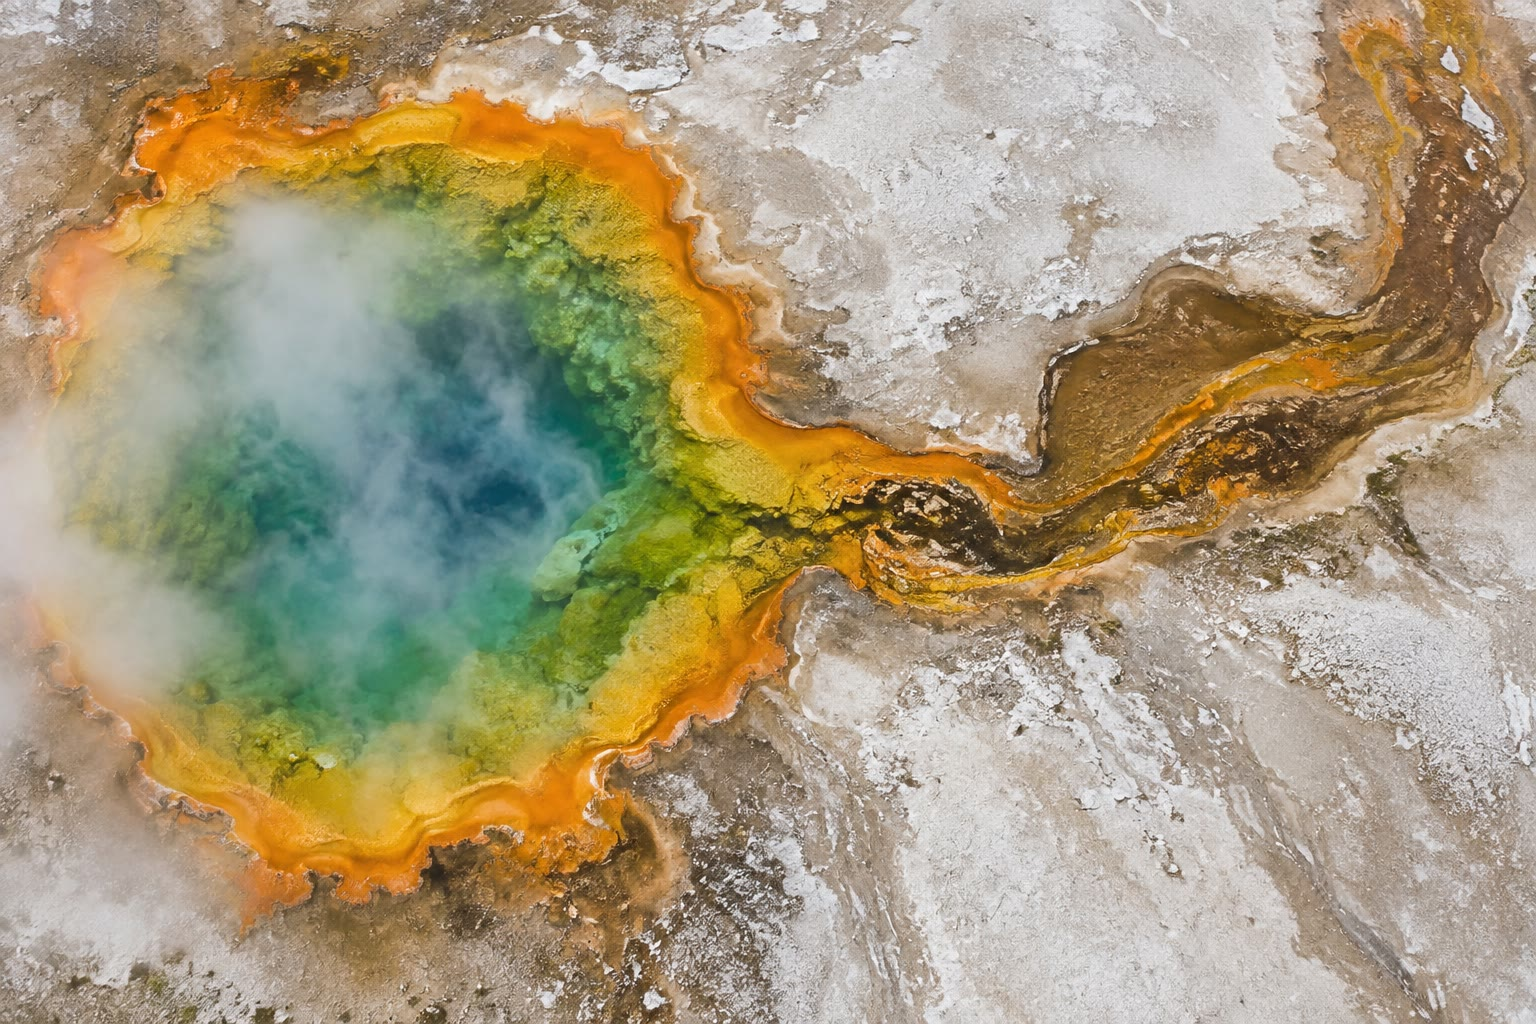
\includegraphics[width=0.62\linewidth]{images/book4/ai/b4-02-hot-spring-mats.jpg}

{\small 温泉周围的微生物席：每种颜色代表一个
种群，各自生活在其条带对应的温度与化学环境中——
较凉的流出水中为嗜热蓝细菌和绿色细菌，
最热的水中则为无色化能\omterm{def:b2:microbial-metabolism:trophic}{无机营养生物}。}
\end{omfigure}

\begin{remark}[微生物席与早期地球]\label{rem:b2:microbial-metabolism:mats}
在温泉周围和潮间带，层状微生物席厚度仅数毫米，
却将整个柱状结构压缩至光能穿透的厚度：顶层为蓝细菌，
其下为紫色细菌，底部为\omterm{def:b2:microbial-metabolism:anaerobic}{硫酸盐还原}菌，
每一层都消耗其上一层所产生的物质，
而微生物席则随其所截留的沉积物向上迁移。
化石微生物席——叠层石——是最古老的生命证据，
距今 35 亿年。长达二十亿年间，在植物或动物出现之前，
生物圈便是这些微生物席及其上方的浮游生物，
正是它们使空气中充满了氧气，
（\cref{ch:b2:biogeochemical-cycles}）。
\end{remark}

\section{练习}

\begin{exercise}[$\star$]\label{exo:b2:microbial-metabolism:1}
按能源、电子来源和碳源对下列生物分类：一种蓝细菌；
\emph{Nitrosomonas}；以葡萄糖为营养的\emph{E.~coli}；
在光照下以琥珀酸盐生长的一种紫色非硫细菌；
在黑暗中以 $\mathrm{H_2S}$ 为底物的\emph{Thiobacillus}。
\end{exercise}

\begin{exercise}[$\star$]\label{exo:b2:microbial-metabolism:2}
按电子受体在呼吸中的能量产出从高到低排列，
并说明每种受体在沉积物中的哪一层被利用。
\end{exercise}

\begin{exercise}[$\star$]\label{exo:b2:microbial-metabolism:3}
配平葡萄糖被氧化为 $\mathrm{CO_2}$、硝酸盐
被还原为 $\mathrm{N_2}$ 的反应（酸性溶液中，另一产物为水）。
每个葡萄糖需要多少个硝酸根离子？
\end{exercise}

\begin{exercise}[$\star$]\label{exo:b2:microbial-metabolism:4}
定义\omterm{def:b2:microbial-metabolism:biofilm}{生物膜}，并说出它的四个阶段。
举出三个\omterm{def:b2:microbial-metabolism:biofilm}{生物膜}与人类健康或工业相关的场合。
\end{exercise}

\begin{exercise}[$\star\star$]\label{exo:b2:microbial-metabolism:5}
计算 $\Delta G^{\circ\prime}$，其中反应为 $4\mathrm{H_2} + \mathrm{CO_2}
\to \mathrm{CH_4} + 2\mathrm{H_2O}$，所用电位为
$\mathrm{2H^+/H_2}$（\qty{-0.42}{V}）和 $\mathrm{CO_2/CH_4}$
（\qty{-0.24}{V}）。按 \qty{50}{kJ/mol} 计，产甲烷菌每消耗一个 $\mathrm{H_2}$
至多能合成多少个 ATP？评论其生长速率。
\end{exercise}

\begin{exercise}[$\star\star$]\label{exo:b2:microbial-metabolism:6}
某细菌的 $\mu_{\max} = \qty{1.2}{h^{-1}}$，葡萄糖的 $K_s =
\qty{5}{mg/L}$。计算其在葡萄糖浓度为
1、5 和 \qty{50}{mg/L} 时的 $\mu$ 及\omterm{def:b2:unicellular-diversity:division}{世代时间}。它在浓度为多少时以
最大速率的 \qty{90}{\%} 生长？
\end{exercise}

\begin{exercise}[$\star\star$]\label{exo:b2:microbial-metabolism:7}
某\omterm{thm:b2:microbial-metabolism:chemostat}{恒化器}的 $\mu_{\max} = \qty{0.8}{h^{-1}}$，$K_s =
\qty{0.05}{g/L}$，$S_{\text{入}} = \qty{5}{g/L}$，$Y = 0.4$，以
$D = \qty{0.4}{h^{-1}}$ 运行。计算 $S^*$、$X^*$，以及
每升每小时的生物量输出和冲洗速率。
\end{exercise}

\begin{exercise}[$\star\star$]\label{exo:b2:microbial-metabolism:8}
将一个 $\mathrm{NH_4^+}$ 氧化为亚硝酸盐可释放 \qty{275}{kJ}；
硝化细菌以 ATP（\qty{50}{kJ/mol}）的形式捕获其中四分之一，
而将一个 $\mathrm{CO_2}$ 固定为生物量需消耗相当于
12 个 ATP 的能量。每固定一个碳，它必须氧化多少个铵根离子？
与异养生物相比，硝化细菌的产率为何如此之低？
\end{exercise}

\begin{exercise}[$\star\star$]\label{exo:b2:microbial-metabolism:9}
计算\omterm{def:b2:microbial-metabolism:biofilm}{生物膜}中氧气的穿透深度，已知 $D_e =
\qty{1.2e-9}{m^2/s}$，$c_0 = \qty{0.20}{mol/m^3}$，$q =
\qty{0.5}{mol/m^3/s}$。若主体溶液中的氧气浓度加倍，$L_p$ 会
如何变化？若细胞呼吸速率加快为四倍，又会如何？
\end{exercise}

\begin{exercise}[$\star\star\star$]\label{exo:b2:microbial-metabolism:10}
自上而下预测 Winogradsky 柱中的各条带，并说出
每个条带的代谢类型，然后解释：(a) 紫色条带为何形成于其所在位置；
(b) 泥浆为何变黑；(c) 该柱在何种意义上是
封闭系统，在何种意义上又是开放系统。
\end{exercise}

\begin{exercise}[$\star\star\star$]\label{exo:b2:microbial-metabolism:11}
密度为 $n$（每升细胞数）的种群中，每个细胞
以每秒 $p = 5$ 个分子的速率分泌\omterm{prop:b2:microbial-metabolism:quorum}{自诱导物}；该分子
以速率 $k = \qty{5e-4}{s^{-1}}$ 降解。
将稳态浓度 $A^*$ 写成 $n$ 的函数。受体
在 $A_c = \qty{10}{nmol/L}$ 时开启：计算以每毫升细胞数
表示的阈值密度。将其与高密度培养物（每毫升 $10^{9}$ 个）
和海水（每毫升 $10^{5}$ 个）进行比较，并解释
为何在悬浮体系中永远达不到\omterm{prop:b2:microbial-metabolism:quorum}{群体感应}的体积里，
\omterm{def:b2:microbial-metabolism:biofilm}{生物膜}却能达到\omterm{prop:b2:microbial-metabolism:quorum}{群体感应}。
\end{exercise}

\begin{exercise}[$\star\star\star$]\label{exo:b2:microbial-metabolism:12}
“\omterm{def:b2:unicellular-diversity:prokaryote}{原核生物}主导着地球的化学过程。”请结合本章中三个
真核生物无法完成的过程进行讨论，并分别说明
一旦该过程停止，生物圈将会发生什么。
\end{exercise}

\section{问题：一座污水处理厂}

\begin{problem}[{周末问题——将某镇的污水处理厂视为一组微生物反应器进行分析，
从细菌的能量学讲起，直至为其提供动力的甲烷，
最后落到工厂的能量平衡上}]
\label{pb:b2:microbial-metabolism:1}
某工厂每天处理 $Q = \qty{10000}{m^3}$ 污水，污水中含有
\qty{300}{g/m^3} 有机物（以燃烧它所需的氧量计，
即其\emph{化学需氧量}，COD），以及
\qty{40}{g/m^3} 铵态氮。该厂设有一个曝气的
活性污泥池、一个用于反硝化的缺氧池，以及一个
用于污泥的厌氧消化池。数据如下：好氧异养生物
以产率 $Y = 0.4$ 转化有机物
（按千克计，每千克底物 COD 生成生物量 COD，其余部分被氧化）；
\omterm{prop:b2:microbial-metabolism:lithotrophy}{硝化作用}每千克氮需要 \qty{4.57}{kg} 的 $\mathrm{O_2}$；
\omterm{def:b2:microbial-metabolism:anaerobic}{反硝化作用}每千克硝酸盐氮需要 \qty{2.86}{kg} 底物 COD；
曝气每千瓦时输送 \qty{2}{kg} 的
$\mathrm{O_2}$；污泥中的 COD 在消化池中以
\qty{60}{\%} 的比例转化为甲烷，每千克转化的 COD
生成 \qty{0.35}{m^3} 甲烷，其能量含量为
\qty{36}{MJ/m^3}，在电效率为 \qty{35}{\%} 的发电机中燃烧。
硝化细菌：$\mu_{\max} = \qty{0.5}{d^{-1}}$，$K_s =
\qty{1}{g/m^3}$，以铵态氮计。

\medskip
\noindent\textbf{第一部分——能量学。}
\begin{enumerate}
  \item 利用\omterm{thm:b2:microbial-metabolism:redox}{电子塔}，计算 $\Delta G^{\circ\prime}$
        对 1 摩尔葡萄糖（24 个电子，电位
        \qty{-0.43}{V}）被氧气（\qty{+0.82}{V}）氧化的过程。
  \item 计算硝酸盐被还原为 $\mathrm{N_2}$
        （\qty{+0.74}{V}）时的标准自由能变化，以及硫酸盐被还原为硫化物
        （\qty{-0.22}{V}）时的标准自由能变化。
  \item 为何反硝化只在缺氧池中开始，
        而\omterm{def:b2:microbial-metabolism:anaerobic}{硫酸盐还原}（伴有恶臭）是工厂运行不良的
        标志？
  \item 若细胞以 ATP（\qty{50}{kJ/mol}）的形式捕获
        自由能的 \qty{40}{\%}，则三种代谢途径各能为
        每个葡萄糖产生多少个 ATP？
  \item 要获得相同的生长量，\omterm{def:b2:microbial-metabolism:anaerobic}{硫酸盐还原}菌需
        比好氧菌多处理多少葡萄糖？
  \item 消化池中的\omterm{def:b2:microbial-metabolism:fermentation}{发酵}菌每个葡萄糖获得 2 个 ATP。试解释
        为何消化池仍几乎不产生生物量，
        而主要产生气体。
\end{enumerate}

\medskip
\noindent\textbf{第二部分——曝气池。}
\begin{enumerate}[resume]
  \item 计算每日有机物负荷，
        以千克 COD 表示。
  \item 计算每日产生的生物量（以 COD 表示），以及
        氧化其余有机物所需的氧量。
  \item 计算处理这些有机物所需的曝气能量，
        以千瓦时每天计。
  \item 计算每日氮负荷，以及硝化
        这些氮所需的氧量。
  \item 污泥在池中的平均停留时间为 $\theta$
        （即其\omterm{thm:b2:microbial-metabolism:chemostat}{稀释速率}的倒数）。$\theta$ 低于多少时，
        无论铵浓度为多少，硝化菌都会被冲出系统？
  \item 取 $\theta = \qty{10}{d}$，计算
        出水中残余铵浓度。
  \item 冬季将 $\mu_{\max}$ 降至 \qty{0.25}{d^{-1}}。重新计算
        残余铵浓度，并说明运行人员应采取什么措施。
\end{enumerate}

\medskip
\noindent\textbf{第三部分——反硝化与消化池。}
曝气池中生成的硝酸盐被回流至缺氧池，
在那里异养菌利用进入的有机物将其还原。
\begin{enumerate}[resume]
  \item 计算反硝化全部氮所消耗的有机物
        量（以千克 COD 每天计）。
  \item 计算每日释放到空气中的氮质量，
        即 $\mathrm{N_2}$ 的日排放量，以及出水中以铵形式排出的氮质量
        （问题 12）占负荷的分数。
  \item 这部分有机物无需再曝气。计算所节省的
        氧量，以及全厂的总需氧量
        （剩余有机物加\omterm{prop:b2:microbial-metabolism:lithotrophy}{硝化作用}）。
  \item 所产生的污泥（问题 8，以 COD 计）进入
        消化池。计算每日产生的甲烷量。
  \item 计算该甲烷的能量，以及它
        可产生的电量。
  \item 计算满足总需氧量所需的曝气用电量，
        即问题 16 中的总需氧量，并进行比较。
\end{enumerate}

\medskip
\noindent\textbf{第四部分——\omterm{def:b2:microbial-metabolism:biofilm}{生物膜}反应器。}
滴滤池在石块上培养\omterm{def:b2:microbial-metabolism:biofilm}{生物膜}；主体水中
氧含量为 \qty{0.2}{mol/m^3}，$D_e = \qty{1.5e-9}{m^2/s}$，
\omterm{def:b2:microbial-metabolism:biofilm}{生物膜}的呼吸速率为 $q = \qty{0.3}{mol/m^3/s}$。
\begin{enumerate}[resume]
  \item 推导\omterm{def:b2:microbial-metabolism:biofilm}{生物膜}中氧浓度分布 $c(x)$，设膜厚到足以
        出现缺氧。
  \item 计算穿透深度。
  \item \omterm{def:b2:microbial-metabolism:biofilm}{生物膜}厚 \qty{300}{\micro m}。好氧部分占
        多大比例？下层细胞如何利用
        由好氧层向下扩散的硝酸盐？
  \item 解释为何单个\omterm{def:b2:microbial-metabolism:biofilm}{生物膜}能同时进行硝化与
        反硝化，而曝气池则做不到。
  \item 加入氯对出水消毒。给出两个理由，
        说明为何\omterm{def:b2:microbial-metabolism:biofilm}{生物膜}能耐受足以杀死
        悬浮状态下同种细菌的加氯剂量。
  \item 给出结果：全厂每日需氧量、
        甲烷产量，以及甲烷所提供的
        曝气用电量占比。
\end{enumerate}
\end{problem}
